\FloatBarrier
\subsection{RLS identification with step \& white noise inputs}

A crucial component of the RLS implementation in Matlab is illustrated in \autoref{code:RLSISWNIImplementation}. In preceding sections we will adapt the code to accommodate each scenario.

\begin{code}
	\begin{matlabcode}{firstnumber = 12}
	Plot=[1 5 6];
	na =3; nb=2;d=0;Ts=0.3;
	N=max(na+1,nb+d+1);
	for L=1:N
	P{L}=eye(na+nb+1)*10^(6);
	end
	theta_hat(:,1:N)=zeros(na+nb+1,N);
	epslon(1:N)=0;
	y1(1:N)=y(1:N);
	for i=N:length(y)
	for j=1:na
	if i-j <=0
	phiT(i,j)=0;
	else
	phiT(i,j)=[-y(i-j)];
	end
	end
	for j=0:nb
	if i-j-d <= 0
	phiT(i,j+1+na)=0;
	else
	phiT(i,j+1+na)=[u(i-j-d)];
	end
	end
	K{i}=P{i-1}*phiT(i,:)'*inv(1+phiT(i,:)*P{i-1}*phiT(i,:)');
	epslon(i)=y(i)-phiT(i,:)*theta_hat(:,i-1);
	theta_hat(:,i)=theta_hat(:,i-1)+K{i}*epslon(i);
	P{i}=(eye(length(K{i}*phiT(i,:)))-K{i}*phiT(i,:))*P{i-1};
	P{i}=(P{i}+P{i}')/2;
	end
	
	Theta_hat=theta_hat(:,end);
	Gz=tf([Theta_hat(na+1:end)'],[1,Theta_hat(1:na)'],Ts)
	
	for l=1:length(phiT(:,1))
	y1(l)=phiT(l,:)*theta_hat(:,l);
	end
	\end{matlabcode}
	\captionof{listing}{RLS implementation in Matlab}
	\label{code:RLSISWNIImplementation}
\end{code}

To identify the system, we employed RLS with a step input. The effectiveness of the RLS identification is demonstrated in \autoref{fig:RLSISWNIStepResponse} by comparing the measured and predicted system responses. The convergence of the system parameters is detailed in \autoref{fig:RLSISWNIStepResponseParams}, and the final transfer function is provided in \autoref{eq:RLSISWNIStepTransferFunction}.  The low average MSE of $10^{-6}$ with a simple step input is almost meaningless.

\begin{figure}
	\centering
	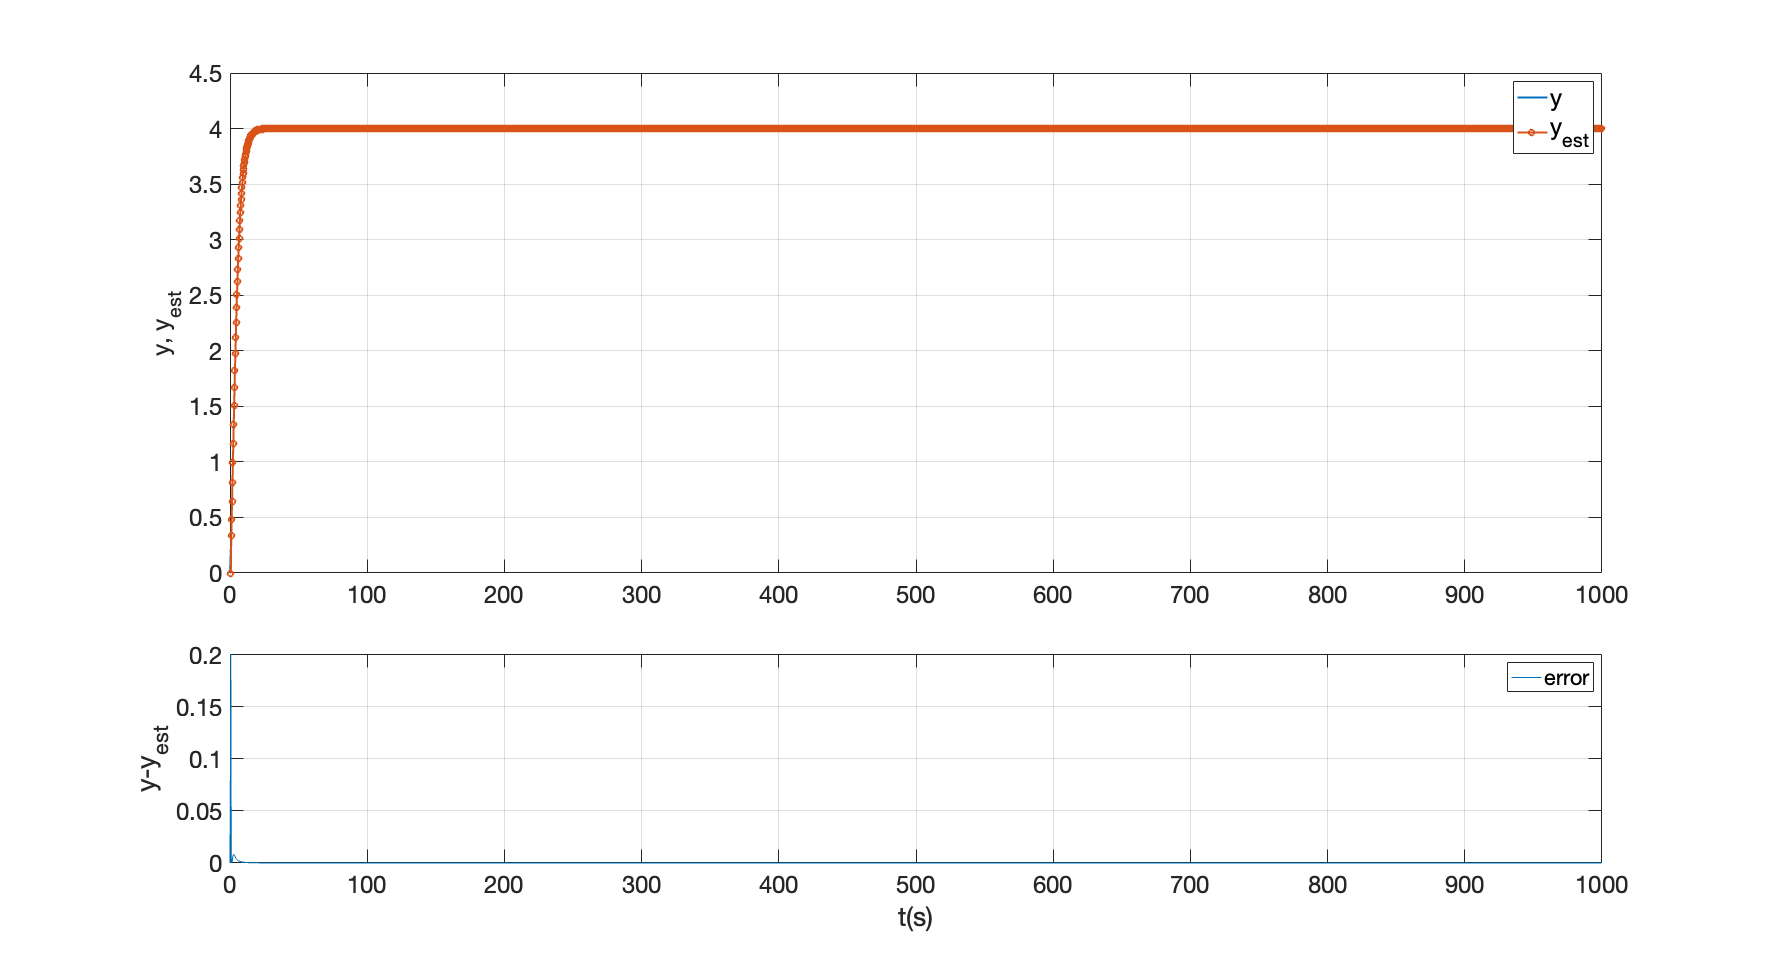
\includegraphics[totalheight=8cm]{images/RLSISWNIStepResponse.png}
	\caption{RLS system output comparison for step input}
	\label{fig:RLSISWNIStepResponse}
\end{figure}
\begin{figure}
	\centering
	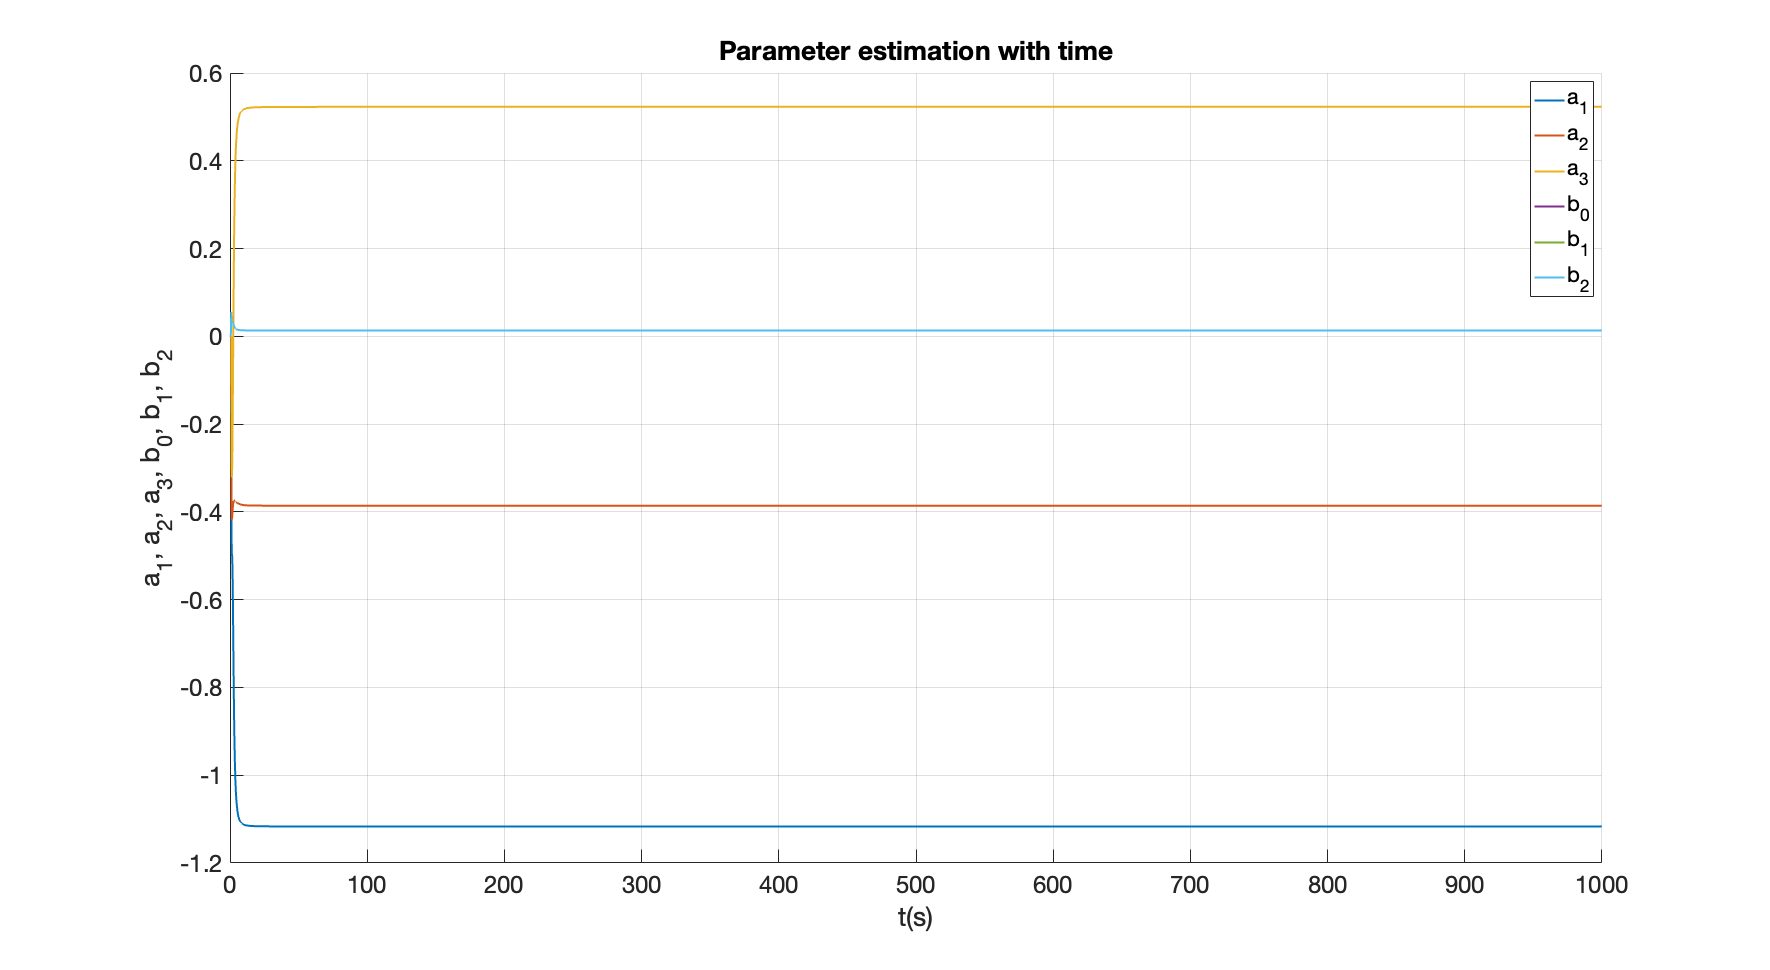
\includegraphics[totalheight=8cm]{images/RLSISWNIStepResponseParams.png}
	\caption{RLS system parameters for step input}
	\label{fig:RLSISWNIStepResponseParams}
\end{figure}
\begin{equation}
	G(z) =	\frac{0.008202 z^2 + 0.008201 z + 0.008202}{z^3 - 1.727 z^2 + 0.6911 z + 0.04855}
	\label{eq:RLSISWNIStepTransferFunction}
\end{equation}

Next, we applied RLS to identify the system using white noise as input. The accuracy of this identification is shown in \autoref{fig:RLSISWNINoiseResponse}, which compares the actual and estimated system outputs. The parameter evolution during the RLS process is detailed in \autoref{fig:RLSISWNINoiseResponseParams}, and the final identified transfer function is given in \autoref{eq:RLSISWNINoiseTransferFunction}. The MSE was approximately $10^{-8}$.

\begin{figure}
	\centering
	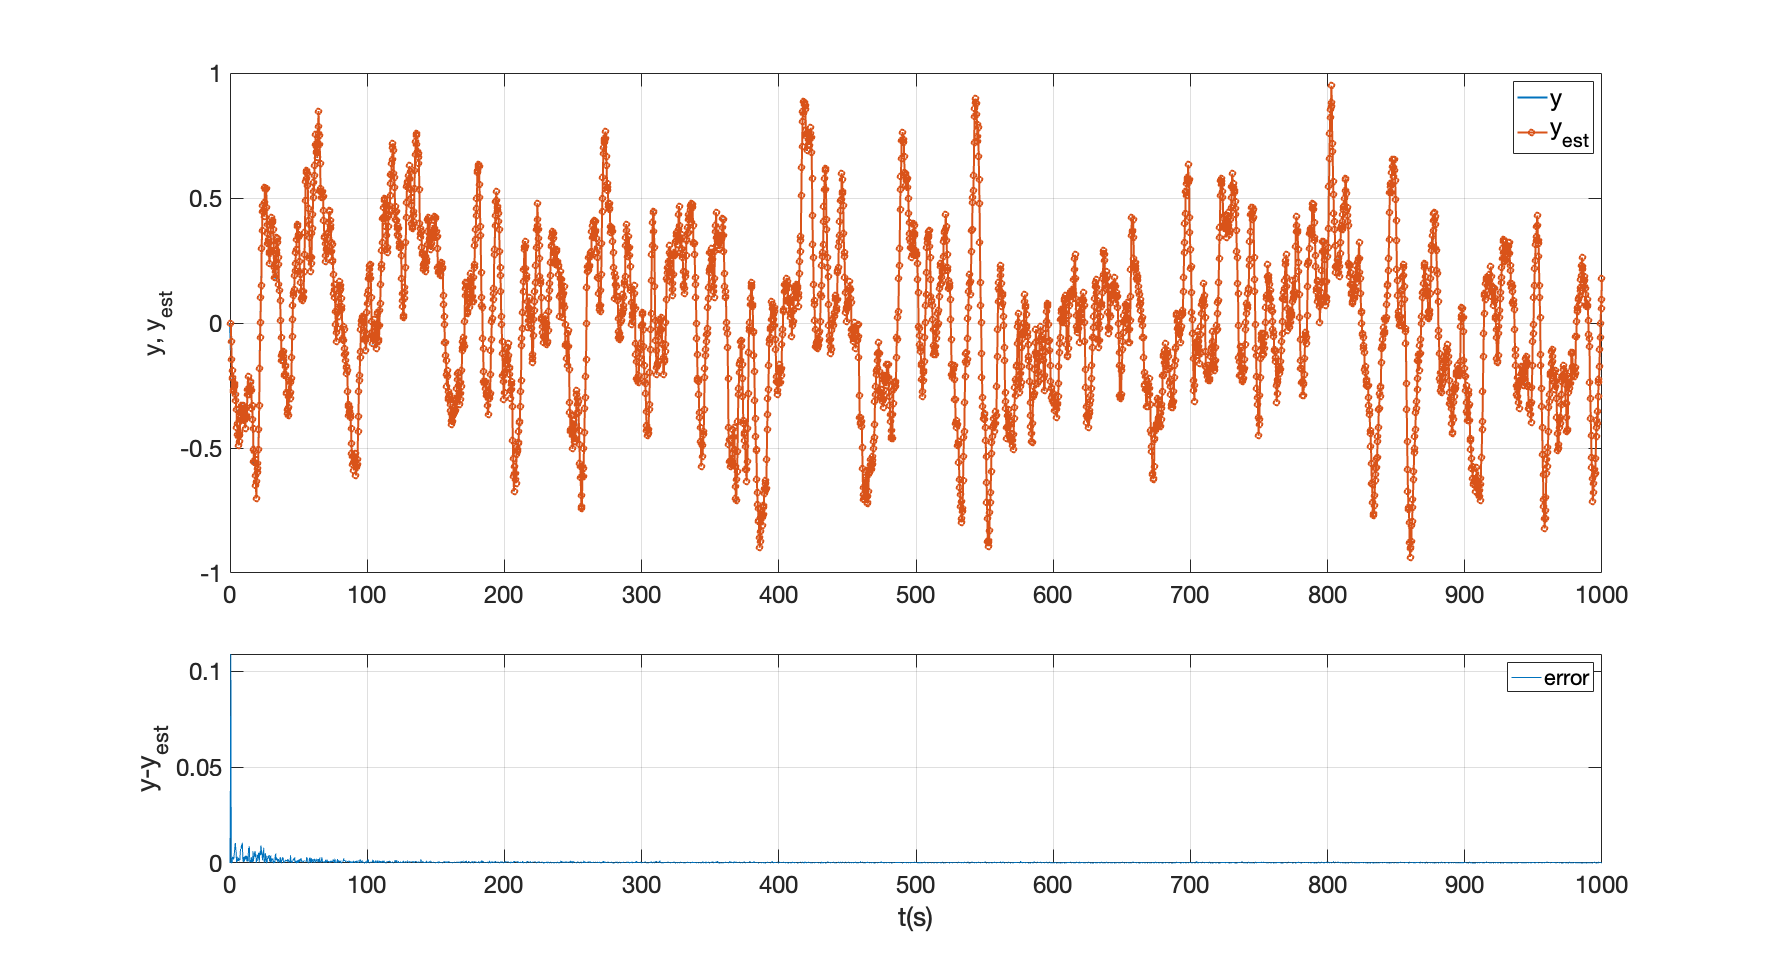
\includegraphics[totalheight=8cm]{images/RLSISWNINoiseResponse.png}
	\caption{RLS system output comparison for noise input}
	\label{fig:RLSISWNINoiseResponse}
\end{figure}
\begin{figure}
	\centering
	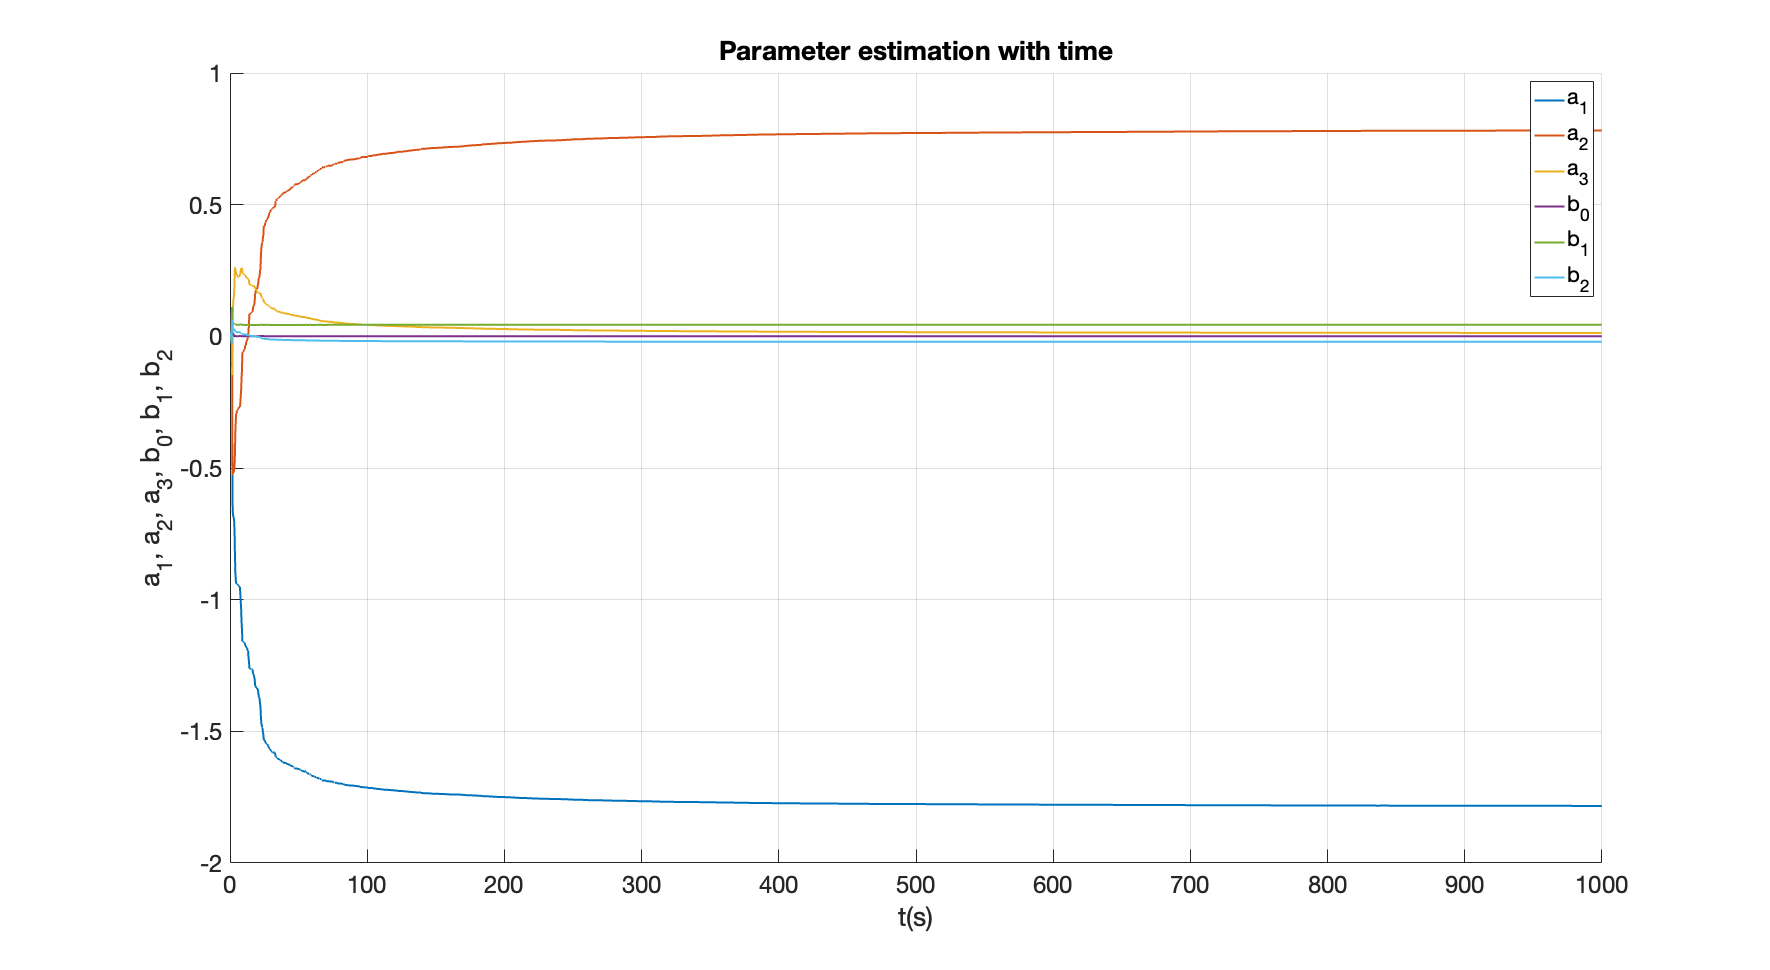
\includegraphics[totalheight=8cm]{images/RLSISWNINoiseResponseParams.png}
	\caption{RLS system parameters for noise input}
	\label{fig:RLSISWNINoiseResponseParams}
\end{figure}
\begin{equation}
	G(z) =	\frac{-3.684e-06 z^2 + 0.04357 z - 0.02131}{z^3 - 1.791 z^2 + 0.7924 z + 0.009529}
	\label{eq:RLSISWNINoiseTransferFunction}
\end{equation}

The Simulink models for both the step and white noise input systems, as illustrated in \autoref{fig:LSISWNIStepSimulinkModel} and \autoref{fig:LSISWNINoiseSimulinkModel}, are available at \lstinline|assignment1/part2/2_1/RLS2_1_Stp.slx| and \lstinline|assignment1/part2/2_1/RLS2_1_NS.slx|, respectively. The corresponding MATLAB scripts for these systems are located at \lstinline|assignment1/part2/2_1/RLS2_1_step.m| (step input) and \lstinline|assignment1/part2/2_1/RLS2_1_noise.m| (white noise input).
